%Version 3.1 December 2024
% ESE 5760 Final Project — SRAM PVT Analysis
%
%%%%%%%%%%%%%%%%%%%%%%%%%%%%%%%%%%%%%%%%%%%%%%%%%%%%%%%%%%%%%%%%%%%%%%
%%                                                                 %%
%% Please do not use \input{...} to include other tex files.       %%
%% Submit your LaTeX manuscript as one .tex document.              %%
%%                                                                 %%
%% All additional figures and files should be attached             %%
%% separately and not embedded in the \TeX\ document itself.       %%
%%                                                                 %%
%%%%%%%%%%%%%%%%%%%%%%%%%%%%%%%%%%%%%%%%%%%%%%%%%%%%%%%%%%%%%%%%%%%%%

\documentclass[pdflatex,sn-mathphys-num]{sn-jnl}% single-column Math/Phys numbered style

%%%% Standard Packages
\usepackage{graphicx}%
\usepackage{multirow}%
\usepackage{amsmath,amssymb,amsfonts}%
\usepackage{amsthm}%
\usepackage{mathrsfs}%
\usepackage[title]{appendix}%
\usepackage{xcolor}%
\usepackage{textcomp}%
\usepackage{manyfoot}%
\usepackage{booktabs}%
\usepackage{algorithm}%
\usepackage{algorithmicx}%
\usepackage{algpseudocode}%
\usepackage{listings}%

\theoremstyle{thmstyleone}%
\newtheorem{theorem}{Theorem}%
\newtheorem{proposition}[theorem]{Proposition}%

\theoremstyle{thmstyletwo}%
\newtheorem{example}{Example}%
\newtheorem{remark}{Remark}%

\theoremstyle{thmstylethree}%
\newtheorem{definition}{Definition}%

\raggedbottom

\begin{document}

\title[SRAM PVT Analysis]{PVT-Aware Evaluation of 6T SRAM Stability, Writability, and Design Tradeoffs}

\author*[1,2]{\fnm{Krishna Karthikeya} \sur{Chemudupati}}\email{krishkc@seas.upenn.edu}

\author[1]{\fnm{Taarana} \sur{Jammula}}\email{taaranaj@seas.upenn.edu}

\author[1,2]{\fnm{Adithya} \sur{Selvakumar}}\email{adisel@seas.upenn.edu}

\affil*[1]{\orgdiv{Department of Electrical and Systems Engineering}, \orgname{University of Pennsylvania}, \orgaddress{\city{Philadelphia}, \state{PA}, \country{USA}}}
\affil[2]{\orgdiv{Department of Physics and Astronomy}, \orgname{University of Pennsylvania}, \orgaddress{\city{Philadelphia}, \state{PA}, \country{USA}}}

\abstract{We evaluate a 6T SRAM bitcell across FF~1.2~V, TT~1.0~V, and SS~1.0~V corners, with SS~0.8~V included where the metric is defined, and bridge the cell-level results to a 128$\times$128, 8-bit, 16:1 column-multiplexed NVSim macro that was independently built and functionally verified in Cadence Virtuoso at 45\,nm. Stability, writability, and read disturb are extracted from butterfly curves and transient measurements, then compared for three optimizations chosen to address the worst-case metric the baseline reveals: negative-bitline write assist for the slow-corner WNM collapse, wordline-underdrive read assist for the binding read SNM and transient read disturb, and high-$V_t$ PMOS pull-up transistors for the hold-window leakage path through the cross-coupled inverter load. At TT, negative bitline reduces WL-to-Q write delay by 54.5\,\%, wordline underdrive raises read SNM by 39.9\,\% and lowers pulse-window read disturb by 57.3\,\%, and the high-$V_t$ pull-up cuts hold-window supply energy by 13.9\,\% with a 10.2\,\% read-SNM penalty driven jointly by a weaker on-side pull-up and a shifted inverter trip point. Macro results are explicitly labeled \emph{Estimated by NVSim}, \emph{Measured in Cadence}, or \emph{Derived proxy} so that array estimates and circuit-level evidence remain clearly separated.}

\keywords{SRAM, 6T bitcell, PVT, SNM, write noise margin, NVSim, high-$V_t$, negative bitline, wordline underdrive}

\maketitle

%-----------------------------------------------------------------------
\section{Introduction}\label{sec:intro}

6T SRAM bitcells are among the most area- and energy-critical structures in modern SoCs, and their reliability is set by a small number of DC and transient margins that are themselves sensitive to process--voltage--temperature (PVT) variation. As supply voltages scale toward subthreshold and as device variability widens at advanced nodes, classical noise margins shrink to a point where read or write operations either fail at slow corners or burn unnecessary energy at fast corners. Cell designers respond with selective threshold-voltage choices and assist circuits, but each assist trades one margin against another, and the trade is itself corner-dependent. A coherent evaluation therefore has to do three things at once: extract the right margin definition for each operating mode, sweep PVT widely enough to expose the binding constraint, and then move the resulting optimization claims onto the array level honestly, without overstating the macro-level impact of a cell-level measurement.

This report follows that structure. A 6T bitcell is sized at the TT~1.0~V, 27$^\circ$C reference operating point and characterized across FF~1.2~V, TT~1.0~V, and SS~1.0~V, with SS~0.8~V included wherever the metric remains defined. The cell-level results are then bridged to a 128$\times$128, 8-bit, 16:1 column-multiplexed NVSim macro that was independently built and functionally exercised in Cadence Virtuoso at 45\,nm. Three optimizations are studied, each selected to address a specific worst-case revealed by the baseline:

\begin{itemize}
\item \emph{Negative-bitline write assist}, targeting the monotonically degrading slow-corner WNM that limits writability at SS~1.0~V.
\item \emph{Wordline-underdrive read assist}, targeting the binding read SNM and the dynamic disturbance of the storage node during the read access window.
\item \emph{High-$V_t$ PMOS pull-up transistors}, targeting the subthreshold leakage path through the cross-coupled inverter load during the hold window.
\end{itemize}

At TT, the measured deltas are 54.5\,\% lower WL-to-Q write delay (negative bitline), 39.9\,\% higher read SNM with 57.3\,\% lower pulse-window read disturb (wordline underdrive), and 13.9\,\% lower hold-window supply energy with a 10.2\,\% read-SNM penalty (high-$V_t$ pull-up). At the array level, only two macro columns move under the bridge — leakage and write latency — and every reported macro number is labeled by its evidence type. The remainder of the report develops these results in order: methodology and evidence labels (Section~\ref{sec:setup}), baseline bitcell stability (Section~\ref{sec:baseline-bitcell}), the three cell-level optimizations (Section~\ref{sec:optimizations}), the bridged macro estimates (Section~\ref{sec:array-results}), the Cadence full-array verification that anchors the bridge (Section~\ref{sec:cadence-verify}), and finally the explicit limitations and evidence boundaries (Section~\ref{sec:limitations}).

%-----------------------------------------------------------------------
\section{Methodology and Evidence Labels}\label{sec:setup}

\subsection{6T cell topology and PVT corners}\label{sec:setup-topology}

The cell under study is a textbook 6T bitcell: two cross-coupled CMOS inverters whose PMOS pull-ups (M1, M2) and NMOS pull-downs (M3, M4) hold the differential storage nodes Q and $\overline{\mathrm{Q}}$, plus two NMOS access transistors (M5, M6) that connect Q and $\overline{\mathrm{Q}}$ to the bitlines BL and $\overline{\mathrm{BL}}$ when the wordline asserts. Every metric reported here exercises a different subset of these devices: hold uses only the inverter loop with the wordline low, read additionally activates the access path while the bitlines are precharged, and write actively forces one bitline against the inverter to flip the cell. Because the three metrics stress different parts of the cell, no single corner pessimization can capture all of them simultaneously, which is the underlying reason the corner sweep is necessary.

Process--voltage variation is exercised at three primary corners — FF at 1.2~V, TT at 1.0~V, and SS at 1.0~V — selected to span the practical envelope without leaving any one corner ambiguous. SS at 0.8~V is added selectively for the metrics that remain extractable under near-threshold operation: hold-window supply energy and write delay are still well defined, but the baseline cell does not have a valid read butterfly at SS~0.8~V because the limiting eye degenerates without an explicit read assist. That degeneration is itself a useful empirical motivation for the wordline-underdrive read assist evaluated in Section~\ref{sec:opt-wlud}.

\subsection{Hold and read SNM via limiting-eye largest-square fit}\label{sec:setup-snm}

Hold SNM and read SNM are both extracted from butterfly curves obtained by sweeping V(Q) while V($\overline{\mathrm{Q}}$) is held at the alternative inverter output. The reported margin is the side length of the largest square that fits inside the limiting eye of the butterfly. This largest-inscribed-square convention reduces the two-dimensional butterfly geometry to a single conservative number per corner, which is what makes per-corner comparison across optimizations meaningful. The same fit routine is applied to baseline, high-$V_t$, and wordline-underdrive butterflies, so any difference reported between cases is geometric, not algorithmic.

\subsection{Write noise margin via diagonal-corner convention}\label{sec:setup-wnm}

Write noise margin is evaluated using the diagonal corner convention, where the limiting noise square is placed along the main diagonal of the write butterfly. Under this convention, WNM degrades monotonically as the corner slows because the access transistor weakens relative to the cross-coupled inverter loop — exactly the regime in which a write needs to overpower the storage node. The slow corner therefore becomes the binding writability constraint rather than the nominal corner, and the headline writability number is taken at SS~1.0~V rather than TT.

\subsection{Read disturb as a pulse-window transient metric}\label{sec:setup-disturb}

Wordline-underdrive read disturb is reported as a pulse-window transient excursion of the complementary storage node during a read pulse, not as a DC quantity. The intent of an underdrive assist is to suppress the dynamic disturbance the storage node experiences while the access transistor briefly couples it to a precharged bitline, and that disturbance is fundamentally transient: a static SNM by itself does not capture the entire benefit. The pulse-window metric integrates the disturbance over the actual read access window and is reported alongside the DC read SNM.

\subsection{Cadence-to-NVSim bridge and evidence labels}\label{sec:setup-bridge}

The cell-level results bridge to a 128$\times$128, 8-bit, 16:1 column-multiplexed NVSim macro at 45\,nm. NVSim does not directly model any of the three optimizations evaluated here, so each macro quantity is labeled by its source of evidence:

\begin{itemize}
\item \emph{Measured in Cadence}: extracted directly from a bitcell DC or transient simulation.
\item \emph{Estimated by NVSim}: copied from the locked baseline macro run.
\item \emph{Derived proxy}: a baseline NVSim macro quantity scaled by a TT Cadence ratio when the optimization affects a macro column that NVSim cannot model directly.
\end{itemize}

The bridge is intentionally narrow. Only two macro columns move: high-$V_t$ scales the macro leakage column, and negative bitline scales the macro write-latency column. Wordline underdrive does not propagate to a macro column at all, because its defended benefit (cell-level read stability and reduced transient disturb) cannot be projected onto an NVSim quantity without a separate full-array simulation that was not run in the present study. All other macro quantities remain pinned to the locked NVSim baseline.

%-----------------------------------------------------------------------
\section{Baseline Bitcell Stability and Writability}\label{sec:baseline-bitcell}

The baseline cell sets the constraints that motivate each of the three optimizations evaluated in Section~\ref{sec:optimizations}. Across the corner sweep the picture is consistent: hold is comfortable, read is the smallest static margin, and write is the binding constraint at the slow corner.

\begin{figure*}[t]
\centering
\begin{minipage}[t]{0.42\textwidth}
\centering
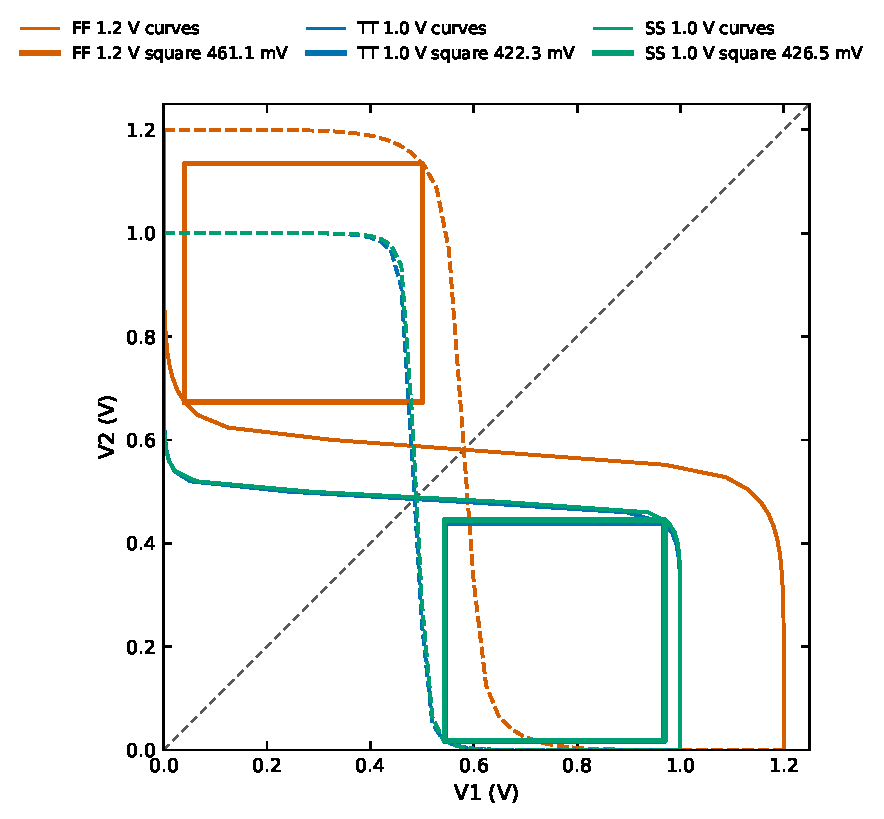
\includegraphics[width=\textwidth]{figures/baseline_hold_snm_all_corners.pdf}
\end{minipage}\hfill
\begin{minipage}[t]{0.42\textwidth}
\centering
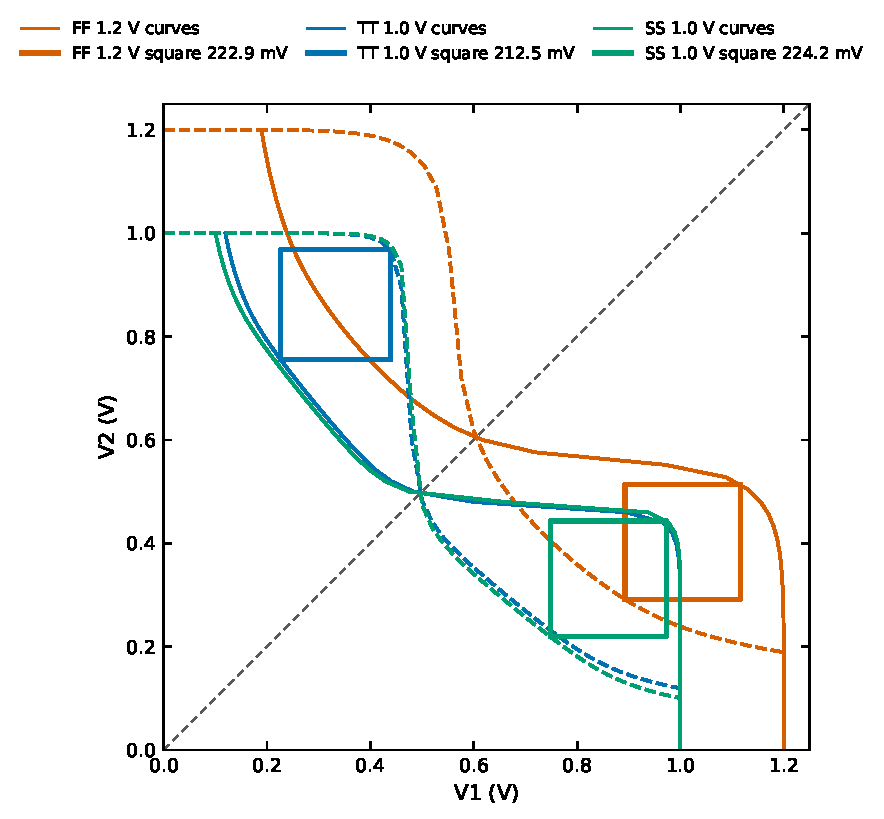
\includegraphics[width=\textwidth]{figures/baseline_read_snm_all_corners.pdf}
\end{minipage}
\caption{Baseline butterfly overlays across corners. Left: hold SNM remains in the 422--461\,mV range; the larger FF eye partly reflects its higher 1.2\,V supply rather than a stronger inverter loop alone. Right: read SNM falls to 212--224\,mV when the access transistor pulls on the held storage node, and sets the read-side reliability floor. Both metrics use the largest-inscribed-square limiting-eye convention.}\label{fig:baseline-hold-read}
\end{figure*}

Hold SNM is comfortable across all three corners (461\,mV at FF, 422\,mV at TT, 426\,mV at SS~1.0~V). Hold stresses only the cross-coupled inverter loop with no active access path, and the supply delivers almost no current beyond subthreshold leakage. The slight non-monotonicity (TT lower than FF and SS) is consistent with the higher FF rail expanding the eye and the SS combination remaining statically robust despite reduced device drive. The structural conclusion is that hold stability is not the limiting concern.

Read SNM falls to 223\,mV at FF, 212\,mV at TT, and 224\,mV at SS~1.0~V. The eye contracts because each access transistor briefly conducts current from the precharged bitline to the storage node holding logic-0, raising that node toward the trip point of the opposite inverter. Across the supported corners, TT sets the smallest eye and therefore sets the read-side reliability floor. The baseline cell does not produce a valid read butterfly at SS~0.8~V — the limiting eye degenerates entirely without a read assist — which is itself the empirical motivation for the wordline-underdrive read assist evaluated in Section~\ref{sec:opt-wlud}.

\begin{figure}[t]
\centering
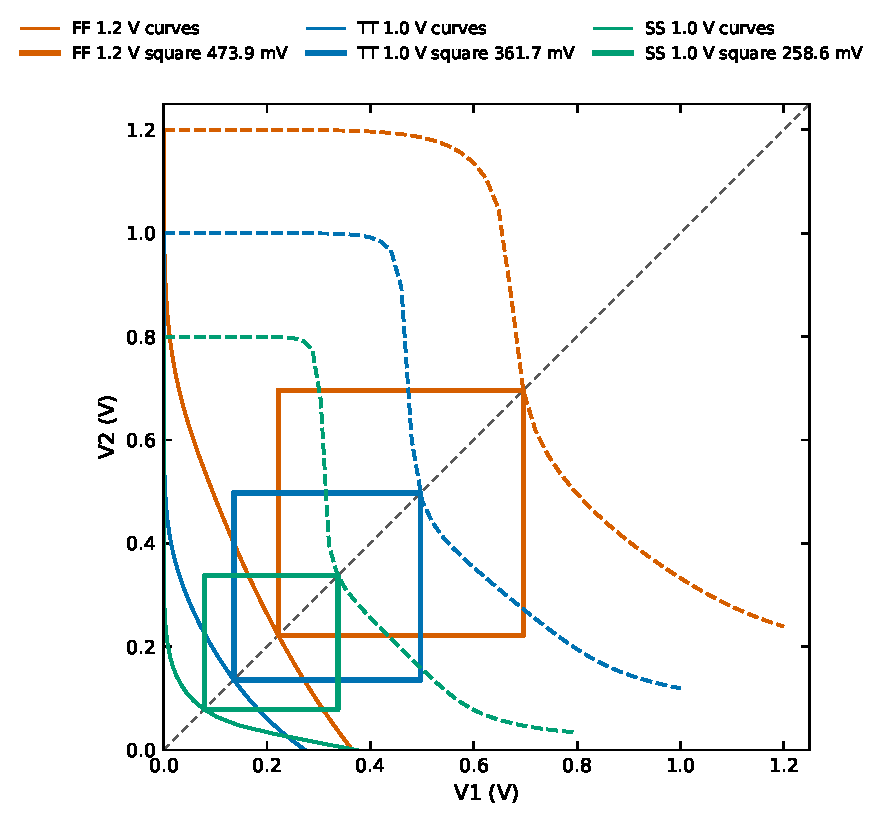
\includegraphics[width=0.92\columnwidth]{figures/baseline_write_nm_all_corners.pdf}
\caption{Baseline write-noise-margin overlays across corners. Under the diagonal-corner convention, WNM drops from 474\,mV at FF, to 362\,mV at TT, to 259\,mV at SS, identifying the slow corner as the binding writability constraint and motivating the negative-bitline write assist evaluated in Section~\ref{sec:opt-negbl}.}\label{fig:baseline-wnm}
\end{figure}

Write noise margin tells a different and more aggressive story: 474\,mV at FF, 362\,mV at TT, and 259\,mV at SS~1.0~V. WNM degrades monotonically as the corner slows because the access transistor weakens relative to the cross-coupled inverter loop — exactly the regime in which the write has to overpower the storage node. The slow corner therefore becomes the writability bottleneck.

In one sentence: hold is fine, read is the smallest static eye and binds at TT, and write is corner-dominated and binds at SS. Each of the three optimizations evaluated next was selected to address one of these three constraints in the order they bind.

%-----------------------------------------------------------------------
\section{Cell-Level Optimizations}\label{sec:optimizations}

The three optimizations are applied to the same baseline cell, and each addresses a specific weakness identified in Section~\ref{sec:baseline-bitcell}. Section~\ref{sec:opt-negbl} attacks the slow-corner WNM collapse with a negative-bitline write assist. Section~\ref{sec:opt-wlud} attacks the binding read SNM and the transient read disturb with a wordline-underdrive read assist. Section~\ref{sec:opt-highvt} attacks the hold-window leakage path through the PMOS pull-up loads with a high-$V_t$ device choice. The pattern across the three is consistent: each assist improves its target metric and concedes elsewhere, with the trade controlled by the corner.

\subsection{Negative-Bitline Write Assist}\label{sec:opt-negbl}

Negative-bitline write assist drives the bitline holding the new data below ground during the write pulse. With BL forced negative, V$_{GS}$ of the access transistor pulling the high storage node down increases beyond the nominal V$_{DD}$, the access path becomes effectively over-driven, and the cross-coupled inverter is flipped earlier in the write window. The benefit is expected to grow as the corner slows, because the baseline access path is exactly the part of the write path that weakens at the slow corner — which is also why the slow corner sets the WNM floor in the baseline cell.

\begin{figure}[t]
\centering
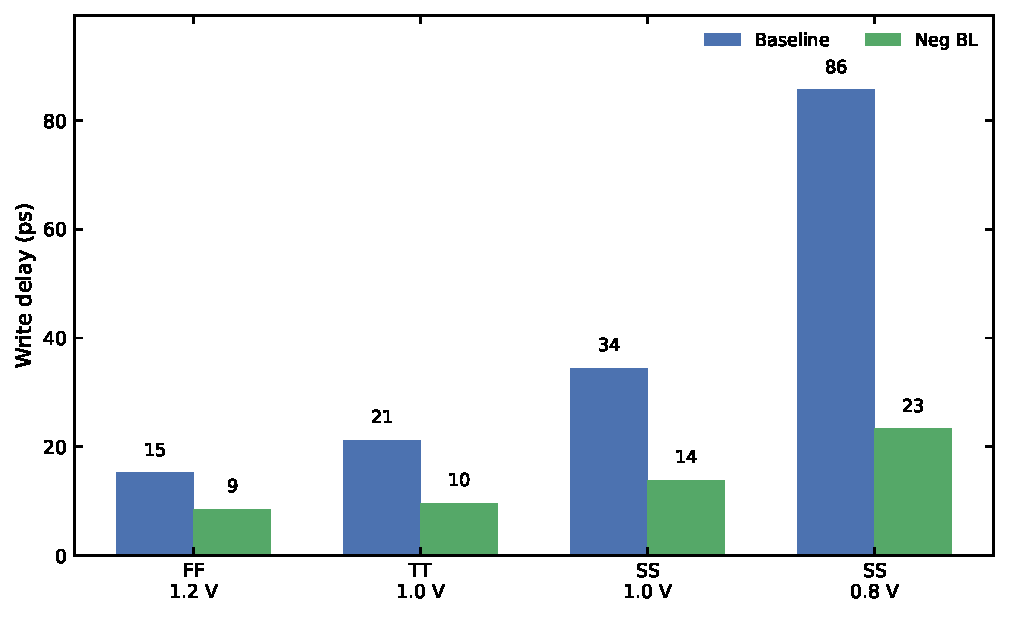
\includegraphics[width=0.95\columnwidth]{figures/negative_bitline_write_delay_by_corner.pdf}
\caption{Per-corner WL-to-Q write delay for the baseline cell versus the negative-bitline assist. TT improves by 54.5\,\%, and the benefit grows monotonically at slower corners, reaching 72.8\,\% at SS~0.8\,V — exactly where the baseline write is most constrained.}\label{fig:negbl-writedelay}
\end{figure}

The measured delay reduction follows the expected profile. WL-to-Q write delay improves by 54.5\,\% at TT and by 72.8\,\% at SS~0.8~V, the worst-case corner under the baseline. This is the desired profile for a write assist: a relatively modest gain at the strong corners where it is not needed, and the largest gain exactly where the baseline cell is weakest. Because the assist is implemented in periphery (a brief negative excursion of the bitline relative to the substrate during the write pulse) rather than in the cell, the cost is paid entirely outside the bitcell footprint and does not perturb hold or read margins.

\begin{figure*}[t]
\centering
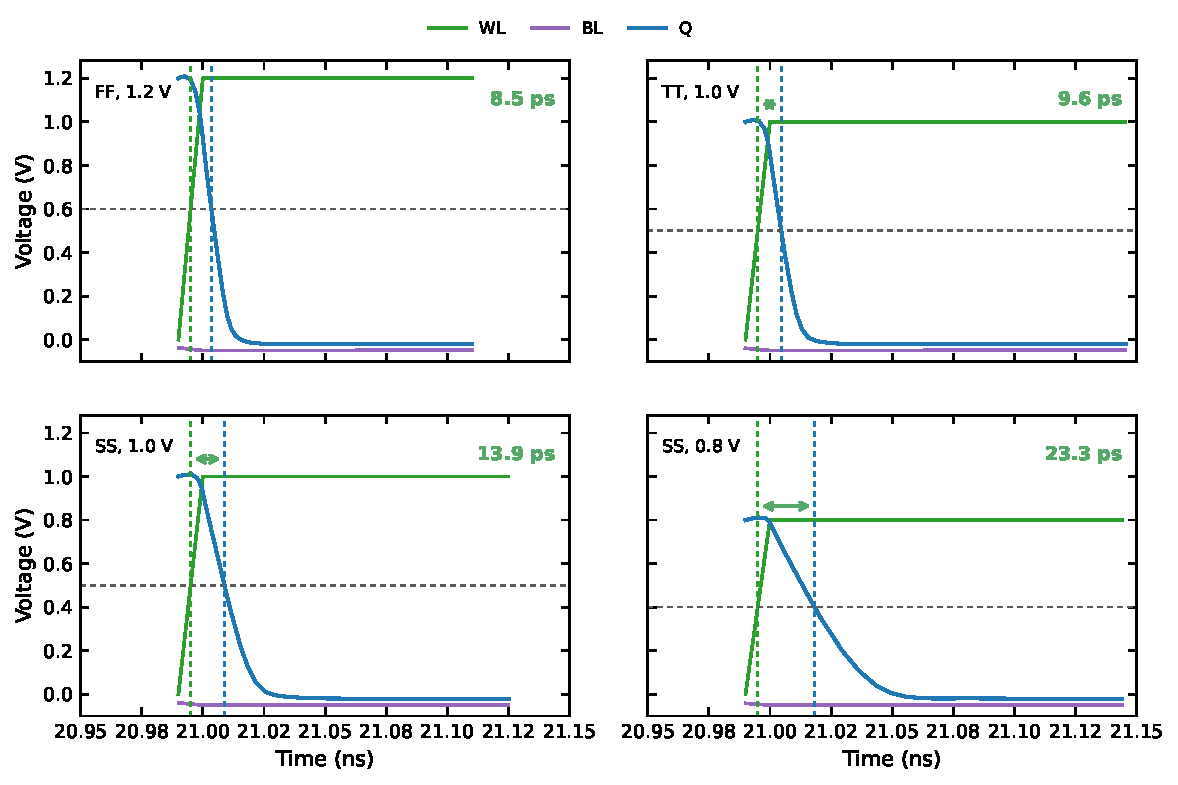
\includegraphics[width=0.82\textwidth]{figures/negative_bitline_write_delay_grid.pdf}
\caption{Per-corner transient write waveforms under the negative-bitline assist. The assisted storage-node transition begins earlier and completes faster than the baseline write at every corner, with the visible gap between baseline and assisted traces widening as the corner slows.}\label{fig:negbl-grid-main}
\end{figure*}

The waveform view confirms that the delay reduction is not an artifact of the threshold-crossing definition: the assisted Q transition leaves the held value earlier and steepens through the metastable region, exactly in the corners where the baseline write is slowest. Combined with the per-corner bar chart in Figure~\ref{fig:negbl-writedelay}, the picture is a write assist that produces a structurally correct corner profile rather than a single TT-only improvement.

\subsection{Wordline-Underdrive Read Assist}\label{sec:opt-wlud}

Wordline-underdrive read assist holds the wordline below the nominal V$_{DD}$ during the read pulse. Reducing V$_{GS}$ of the access transistor weakens it relative to the cross-coupled NMOS pull-down inside the inverter loop, which is the structural condition for read stability: as long as the access transistor cannot lift the low storage node above the trip point of the opposite inverter, the limiting butterfly eye does not collapse and read SNM is preserved. The same mechanism suppresses the dynamic excursion of the storage node during the read access window, which is why the assist improves both the static SNM and the transient pulse-window read-disturb metric.

\begin{figure*}[t]
\centering
\begin{minipage}[t]{0.42\textwidth}
\centering
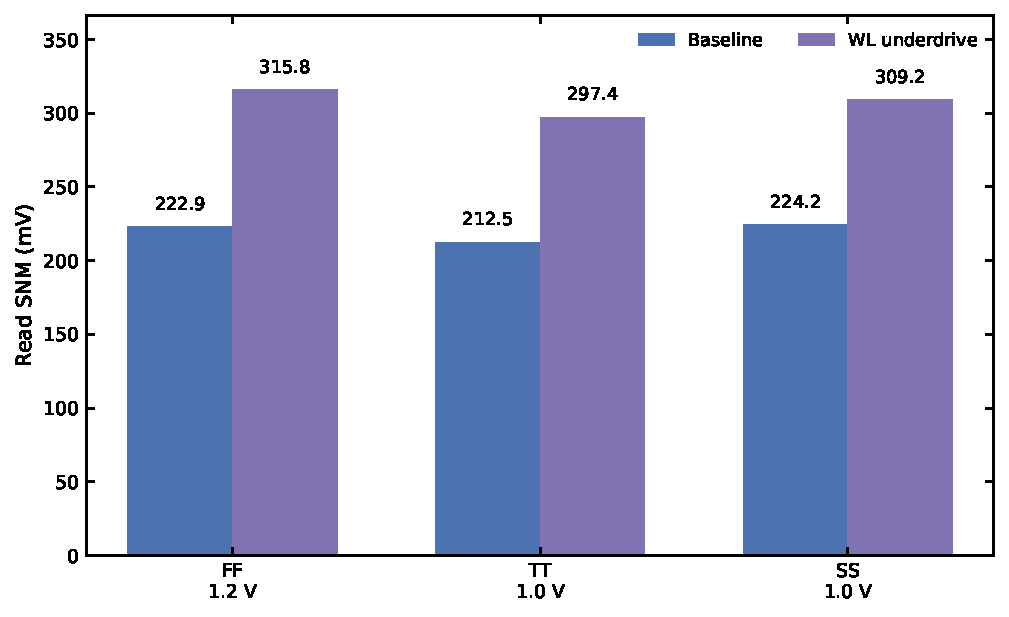
\includegraphics[width=\textwidth]{figures/wordline_underdrive_read_snm_comparison.pdf}
\end{minipage}\hfill
\begin{minipage}[t]{0.42\textwidth}
\centering
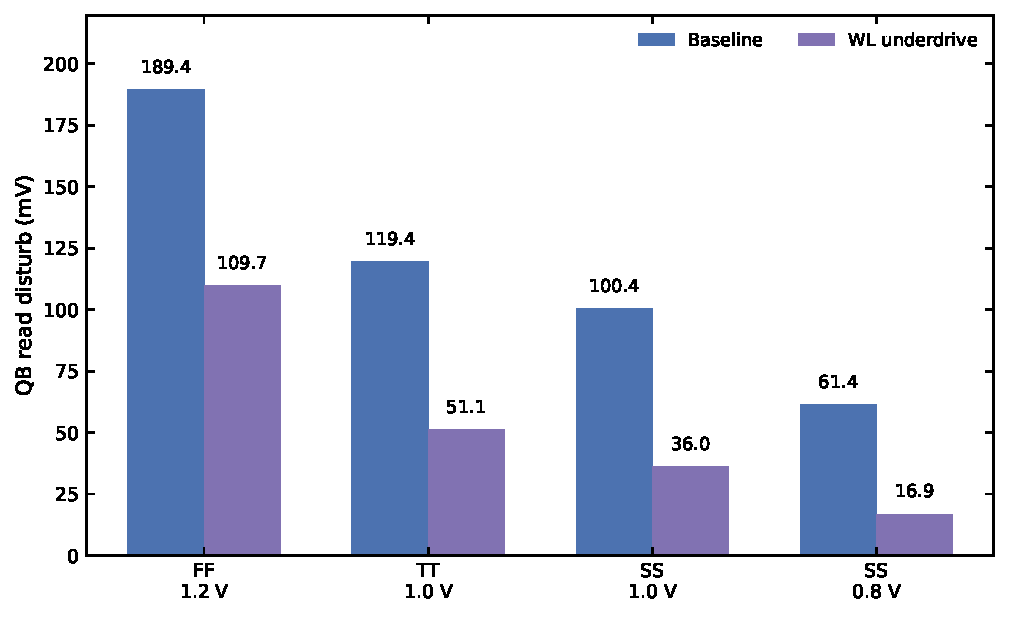
\includegraphics[width=\textwidth]{figures/wordline_underdrive_read_disturb_comparison.pdf}
\end{minipage}
\caption{Wordline-underdrive read assist. Left: per-corner read SNM. Right: pulse-window transient disturb on the complementary storage node. At TT, read SNM improves by 39.9\,\% and read disturb drops by 57.3\,\%. The assist also produces a defined read margin at SS~0.8~V, where the baseline cell does not have a valid read butterfly.}\label{fig:wlud-summary}
\end{figure*}

Quantitatively, read SNM improves by 39.9\,\% at TT and the pulse-window read-disturb metric falls by 57.3\,\%. The static and transient gains are mutually reinforcing: the underdriven access transistor both expands the limiting butterfly eye and shrinks the dynamic excursion that would otherwise erode it during the read window. The cost of the assist is paid in read latency through slower bitline development — a periphery-side cost rather than a cell-area or stability cost — which is why the assist remains in the bitcell section of this report rather than being projected onto a macro column.

\begin{figure}[t]
\centering
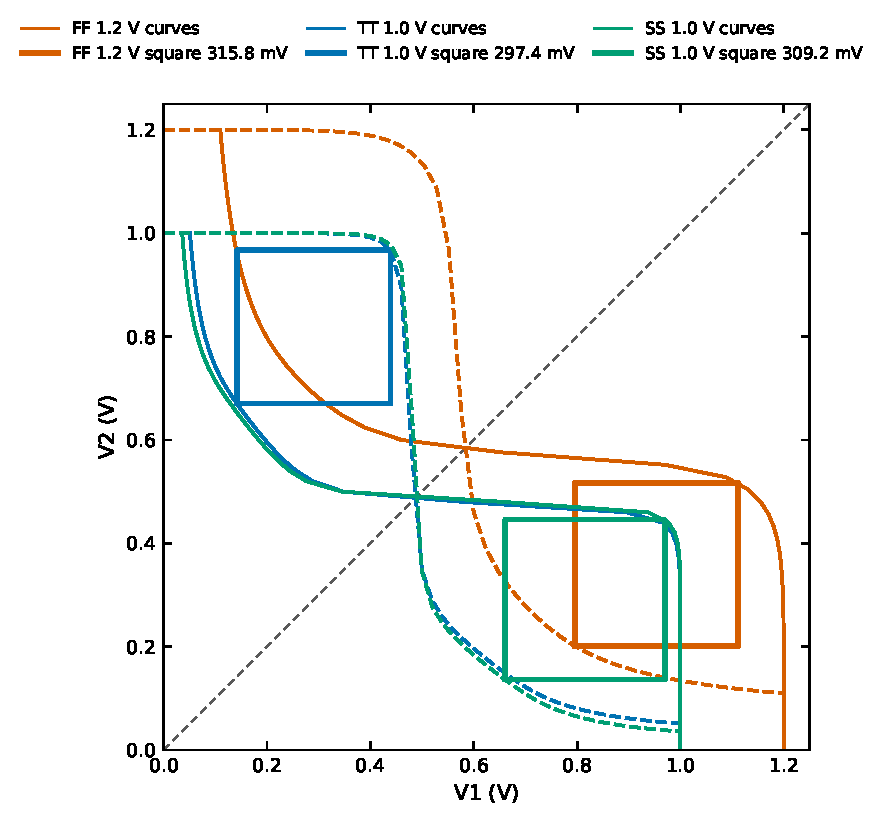
\includegraphics[width=0.95\columnwidth]{figures/wordline_underdrive_read_snm_all_corners.pdf}
\caption{Wordline-underdrive read-SNM butterfly overlays across corners. The limiting eye expands consistently over the corner sweep, with the largest gain at the slow and low-voltage cases where the baseline cell is most read-fragile.}\label{fig:wlud-overlay}
\end{figure}

The overlay view confirms that the gain is not concentrated at a single nominal point. The read eye expands at FF, TT, SS~1.0~V, and SS~0.8~V, with the relative improvement largest at the slow and low-voltage corners — the same direction-of-merit as the negative-bitline write assist above. In both cases the assist helps most exactly where the baseline cell is weakest, which is the structural reason these two assists are the standard pairing for low-voltage 6T arrays.

\subsection{High-$V_t$ PMOS Pull-Up Transistors}\label{sec:opt-highvt}

The third optimization raises the threshold voltage of the two PMOS pull-up transistors (M1, M2) inside the cross-coupled inverter loop. The expected benefit is a reduction in subthreshold leakage through the PMOS load during the hold window: with a higher $|V_{Tp}|$, the off-state PMOS leaks less drain-to-source, and the supply current consumed by the inverter loop while the cell is simply holding state decreases. The expected cost is a small but real reduction in read SNM, driven by two simultaneous mechanisms inside the cell:

\begin{itemize}
\item The high-$V_t$ pull-up is weaker on the on-side of the inverter loop, so the storage node holding logic-1 is held less stiffly against the access transistor that briefly conducts during a read.
\item The inverter trip point shifts toward the lower rail as $|V_{Tp}|$ increases, which compresses the upper lobe of the butterfly and reduces the side length of the limiting square.
\end{itemize}

The two effects act in the same direction and combine into the observed read-SNM penalty. This is structurally different from a high-$V_t$ access-transistor choice, which would weaken the access path during read and therefore \emph{improve} read SNM (effectively a static analog of wordline underdrive). Distinguishing the two is important: they share the words ``high-$V_t$'' but they pull the read margin in opposite directions, and only the pull-up version produces the energy--margin trade reported here.

\begin{figure*}[t]
\centering
\begin{minipage}[t]{0.42\textwidth}
\centering
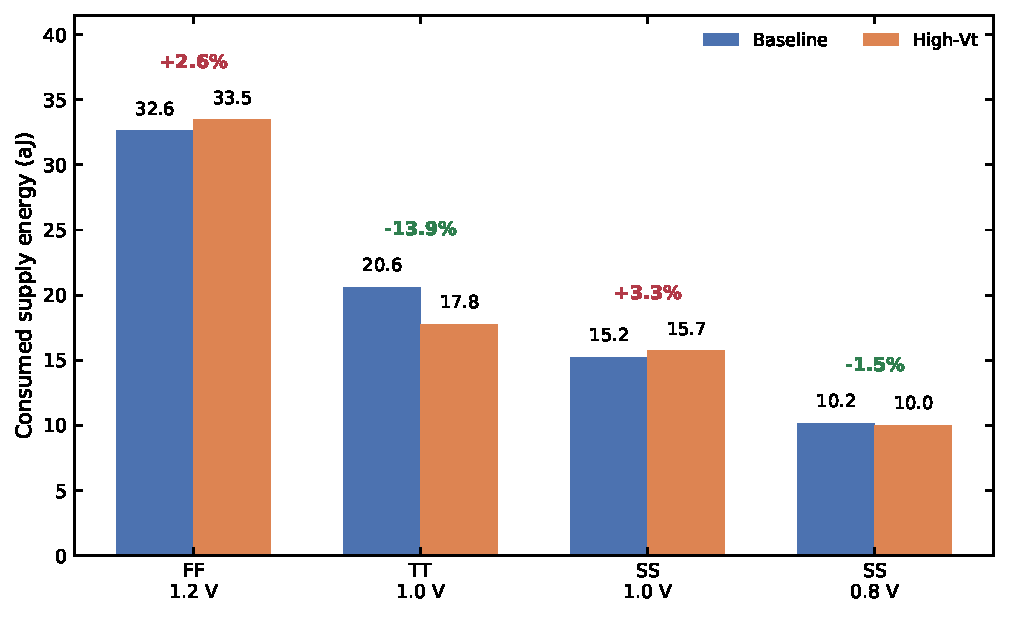
\includegraphics[width=\textwidth]{figures/high_vt_hold_leakage_energy_by_corner.pdf}
\end{minipage}\hfill
\begin{minipage}[t]{0.42\textwidth}
\centering
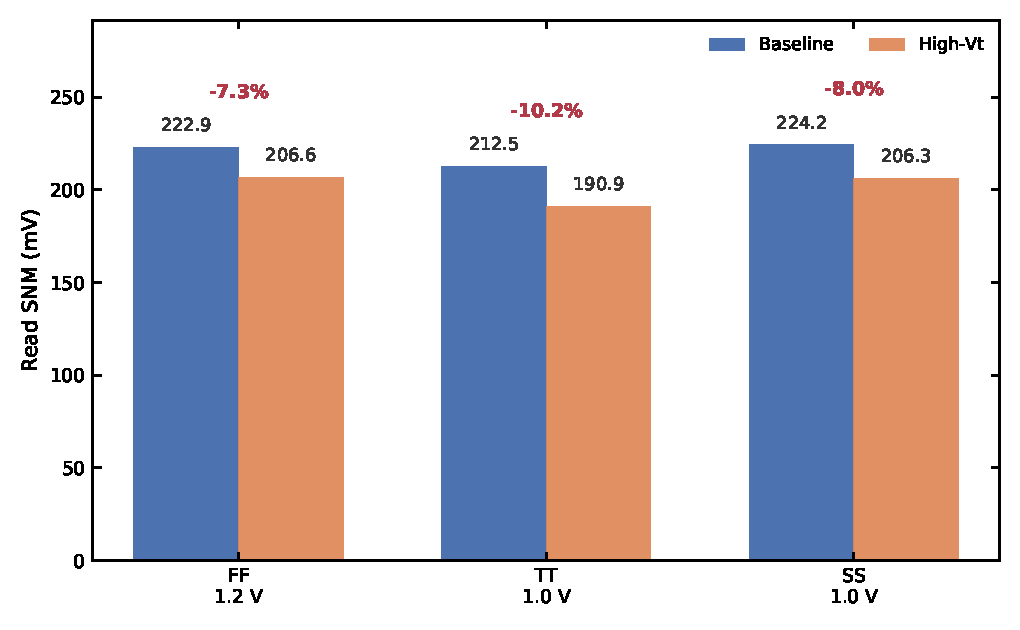
\includegraphics[width=\textwidth]{figures/high_vt_read_snm_by_corner.pdf}
\end{minipage}
\caption{High-$V_t$ pull-up tradeoff across corners. Left: hold-window supply energy integrated over the 6--9\,ns hold segment. Right: read SNM at the three corners where both cells have a valid read butterfly. At TT, hold-window energy improves by 13.9\,\% while read SNM drops by 10.2\,\%. The slight FF energy regression is consistent with gate-tunneling leakage rather than subthreshold leakage dominating at the fast corner, so the high-$V_t$ device choice has weaker subthreshold benefit to offer there.}\label{fig:highvt-summary}
\end{figure*}

At TT, hold-window supply energy drops from 20.6\,aJ to 17.8\,aJ ($-13.9$\,\%) while read SNM drops from 212\,mV to 191\,mV ($-10.2$\,\%). This is the cleanest energy--margin trade in the study: at the nominal corner the leakage path through the PMOS load is the dominant contribution to hold-window supply current, and the high-$V_t$ choice attacks it directly. At FF, the energy figure goes slightly the wrong way, which is the expected behavior of a subthreshold-targeted device choice in a regime where gate-tunneling leakage dominates the static current; SS~1.0~V shows a similarly small energy regression for the same reason. The clean wins are therefore concentrated at TT, which happens to be the corner where leakage matters most for typical retention budgets.

\begin{figure*}[t]
\centering
\begin{minipage}[t]{0.42\textwidth}
\centering
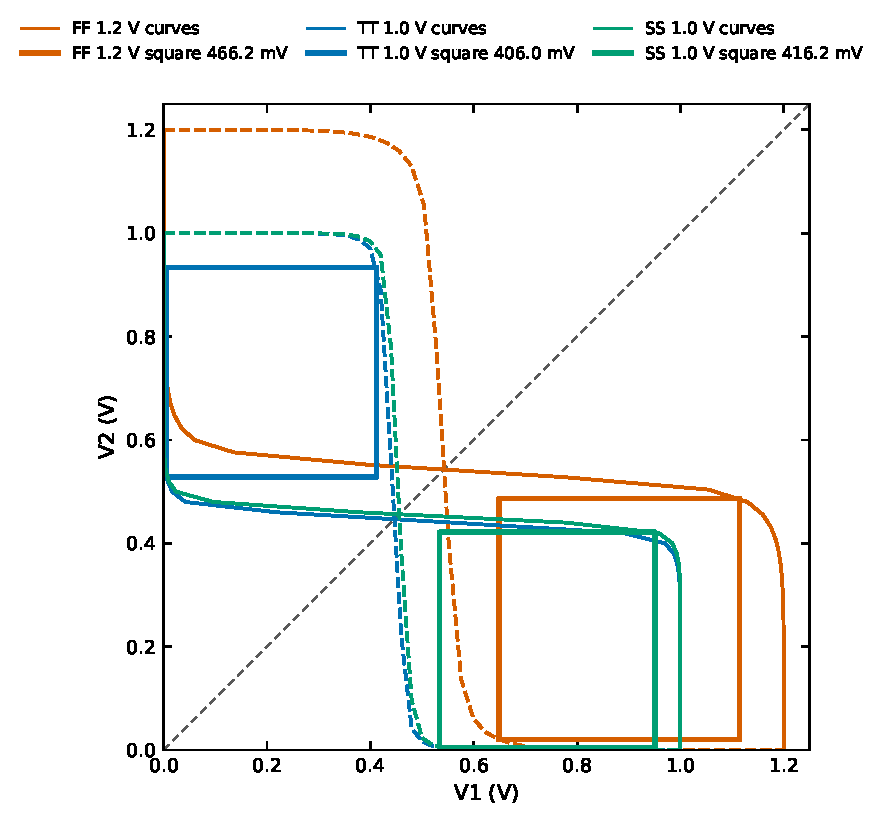
\includegraphics[width=\textwidth]{figures/high_vt_hold_snm_all_corners.pdf}
\end{minipage}\hfill
\begin{minipage}[t]{0.42\textwidth}
\centering
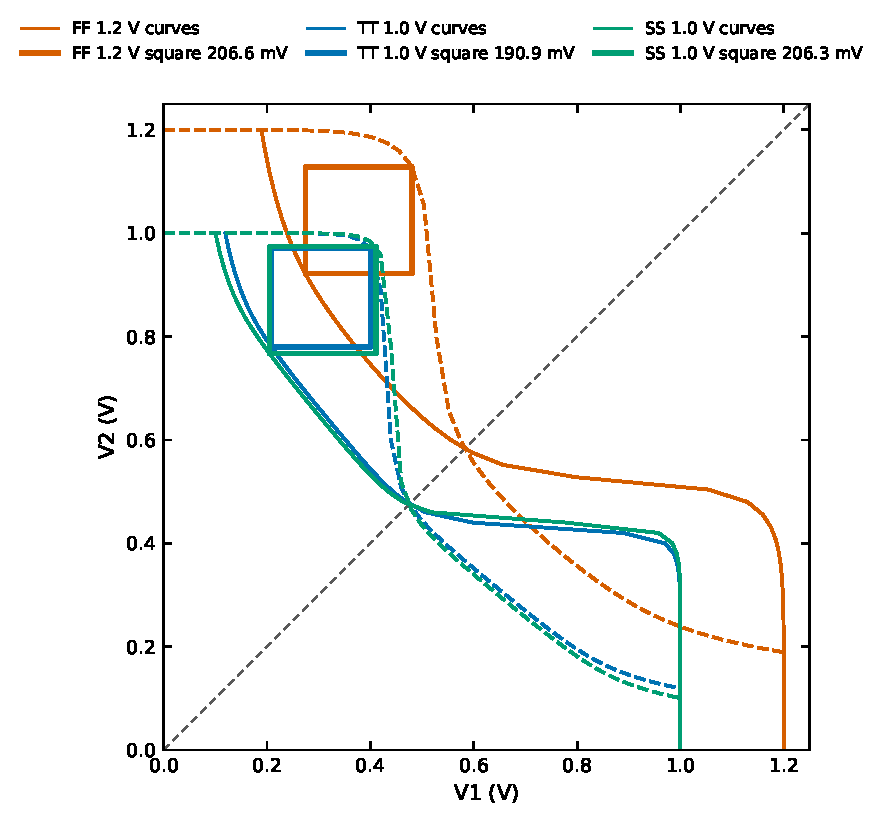
\includegraphics[width=\textwidth]{figures/high_vt_read_snm_all_corners.pdf}
\end{minipage}
\caption{High-$V_t$ pull-up butterfly overlays. Left: hold-state geometry remains close to the baseline across the supported corners — hold is set by the inverter loop holding state with no active access path, which the higher $|V_{Tp}|$ does not significantly alter. Right: the read-side eye contracts at every corner; this is the geometric counterpart of the read-SNM penalty in Figure~\ref{fig:highvt-summary} and reflects the trip-point shift discussed in the prose above.}\label{fig:highvt-overlays}
\end{figure*}

The butterfly view makes the trip-point shift visible directly in the DC geometry. Hold geometry is essentially unchanged at all three corners (hold stresses the inverter loop while it holds state, and the higher $|V_{Tp}|$ does not significantly perturb that equilibrium), while the read-side lobes contract uniformly with the same direction-of-merit as the bar chart above. The summary, then, is that high-$V_t$ pull-up is a clean energy-vs-margin trade at the nominal corner: usable as a leakage knob when retention dominates and stability headroom exists, but neither free at FF or SS, nor available without explicit accounting for the read-SNM penalty.

%-----------------------------------------------------------------------
\section{Array-Level Macro Results}\label{sec:array-results}

The cell-level results bridge to a 128$\times$128, 8-bit, 16:1 column-multiplexed NVSim macro. Only two macro columns move under the present bridge: high-$V_t$ scales macro leakage, and negative bitline scales macro write latency. All other macro quantities remain at the NVSim baseline, and wordline underdrive is intentionally not propagated to any macro number, because its defended benefit is cell-level read stability rather than a macro timing or energy column NVSim can model directly.

\begin{table}[t]
\caption{Baseline NVSim macro summary at the locked 128$\times$128, 8-bit, 16:1 organization. All rows are \emph{Estimated by NVSim}.}\label{tab:nvsim-baseline-macro}
\centering
\begin{tabular}{@{}ll@{}}
\toprule
\textbf{Baseline macro quantity} & \textbf{Value} \\
\midrule
Capacity & 2048~B \\
Physical array & 128 $\times$ 128 \\
Word width & 8~bits \\
Column selection & 16:1 \\
Area & 0.006197~mm$^2$ \\
Read latency & 0.8821~ns \\
Write latency & 0.8821~ns \\
Read energy & 1.3540~pJ \\
Write energy & 0.3210~pJ \\
Leakage & 0.4854~$\mu$W \\
\bottomrule
\end{tabular}
\end{table}

\begin{figure}[t]
\centering
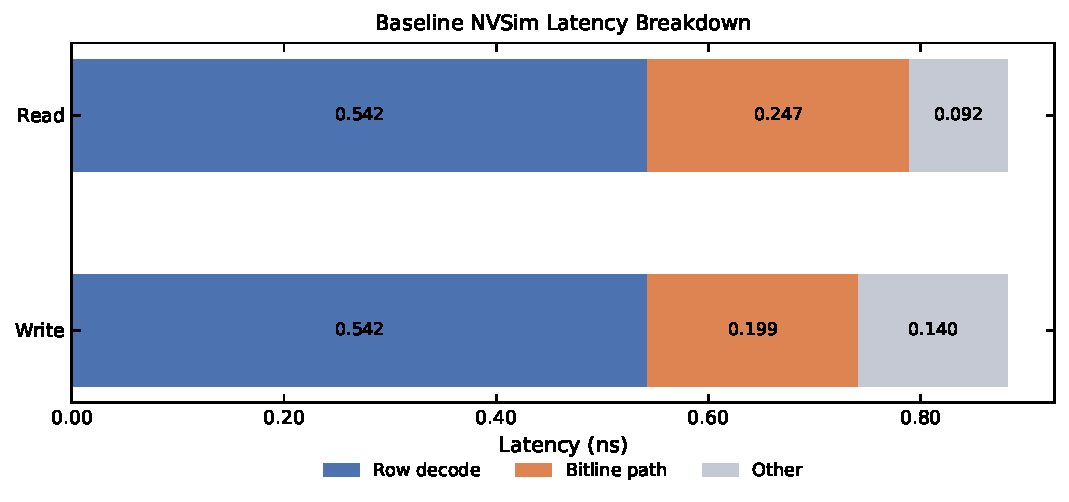
\includegraphics[width=0.95\columnwidth]{figures/baseline_nvsim_latency_breakdown.pdf}
\caption{Baseline macro latency breakdown. Row decode dominates both read and write at approximately 61\,\% of the total 0.8821\,ns access path, so most of the macro access time is outside the part of the path that any cell-level optimization can shorten directly. This is the structural reason a cell-level write assist scales only the bitline-path portion of write latency rather than the full 0.8821\,ns figure.}\label{fig:nvsim-latency-breakdown}
\end{figure}

The latency breakdown is informative for two reasons. First, it explains why even a 54.5\,\% improvement in cell-level write delay does not produce a 54.5\,\% improvement in macro write latency: only the bitline-path portion of the access tree responds to the cell-level write assist, and the dominant row-decode segment is unchanged. Second, it justifies treating row decode and other unrelated macro columns as fixed under the bridge — the only part of the path that the bitcell-level evidence authorizes moving is the part the bitcell-level evidence actually measured.

\begin{figure*}[t]
\centering
\begin{minipage}[t]{0.42\textwidth}
\centering
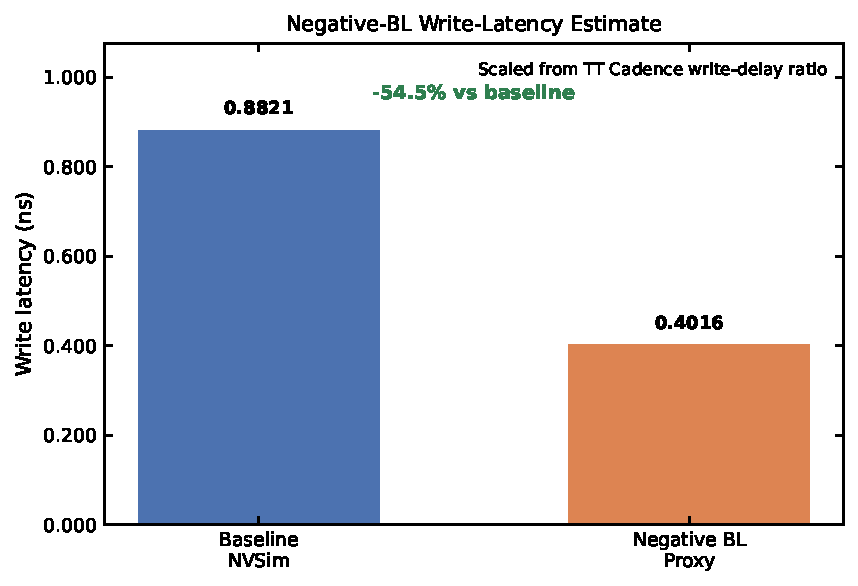
\includegraphics[width=\textwidth]{figures/negative_bl_write_latency_proxy.pdf}
\end{minipage}\hfill
\begin{minipage}[t]{0.42\textwidth}
\centering
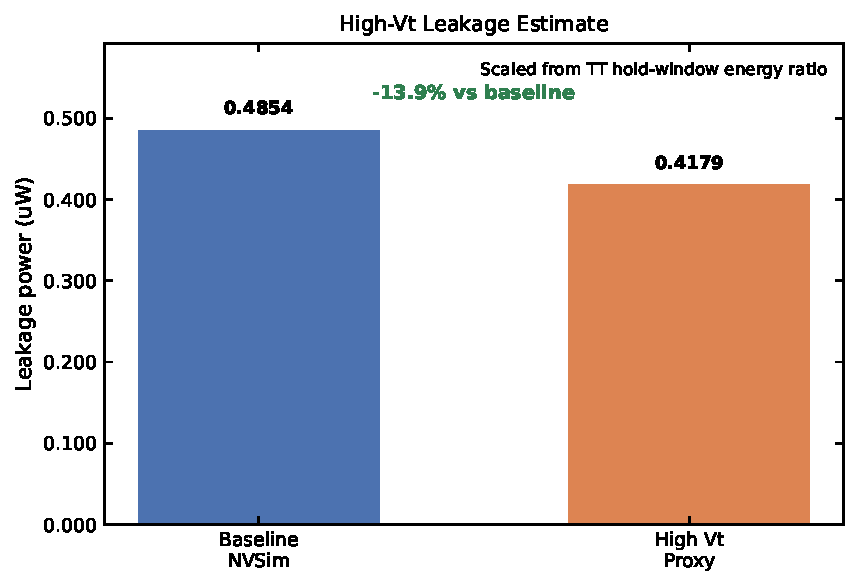
\includegraphics[width=\textwidth]{figures/high_vt_leakage_proxy.pdf}
\end{minipage}
\caption{The two macro columns that move under the present bridge. Left: negative-bitline macro write latency as a derived proxy, scaled by the TT Cadence write-delay ratio: 0.8821\,ns to 0.4016\,ns ($-54.5$\,\%). Right: high-$V_t$ macro leakage as a derived proxy, scaled by the TT hold-window energy ratio: 0.4854\,$\mu$W to 0.4179\,$\mu$W ($-13.9$\,\%). All other macro quantities remain at the NVSim baseline.}\label{fig:array-proxies}
\end{figure*}

The macro story is intentionally narrow. High-$V_t$ pull-up transistors produce a defendable leakage reduction at the macro level. Negative bitline produces a defendable write-latency reduction. Wordline underdrive remains in the bitcell section because its defended benefit — improved read stability and reduced transient disturb — has no direct NVSim column to scale, and faking one would violate the evidence-labeling discipline established in Section~\ref{sec:setup}.

%-----------------------------------------------------------------------
\section{Cadence Full-Array Verification}\label{sec:cadence-verify}

The macro modeled in NVSim was independently built and functionally verified at the schematic level in Cadence Virtuoso at 45\,nm. The 2\,KB array is organized as 128 rows by 128 columns of 6T bitcells, with row decode, column multiplexer, write driver, and sense periphery instantiated around the array. Both the baseline cell and the optimized cells (negative-bitline write driver and underdriven wordline) were inserted into the same array harness, and basic read and write functionality was exercised under TT~1.0~V conditions to confirm that the periphery matches the cell-level expectations established in Sections~\ref{sec:baseline-bitcell} and \ref{sec:optimizations}.

\begin{figure}[h]
\centering
\fbox{\begin{minipage}[c][6cm][c]{0.92\columnwidth}\centering\textit{Cadence Virtuoso schematic of the 128$\times$128 (2\,KB) SRAM array with periphery — drop in screenshot here.}\end{minipage}}
\caption{Cadence Virtuoso 45\,nm schematic of the 128$\times$128 SRAM array with periphery. Both baseline and optimized bitcell variants were instantiated into the same array harness and verified for basic read/write functionality at the TT corner.}\label{fig:cadence-array}
\end{figure}

The full-array build is the empirical anchor for the bridged macro discussion. It establishes that the cell-level numbers reported in this study come from a cell that actually composes into a working 2\,KB array, and that the optimization variants drop into that same array without disturbing the surrounding periphery — a precondition for treating the cell-level Cadence ratios as honest scaling factors for the corresponding NVSim columns. Without this verification step, the derived-proxy macro estimates in Section~\ref{sec:array-results} would be defensible only as device-level claims; with it, they extend to claims about how the macro behaves when the corresponding cell is the one in the array.

%-----------------------------------------------------------------------
\section{Limitations and Evidence Boundaries}\label{sec:limitations}

The evidence boundaries are part of the result, not an afterthought. Stating them explicitly is what allows the rest of the report to be read as a precise claim rather than a generous one.

\begin{itemize}
\item TT nominal is the bridge anchor. Corner robustness remains a cell-level result and is not projected onto the macro. In particular, the FF and SS regressions in the high-$V_t$ hold-energy figure are reported at the cell level only, and not propagated into a corner-dependent macro leakage column.
\item Negative bitline and wordline underdrive were not directly simulated as full-array NVSim cases. Their macro claims are therefore limited to what the present bridge can defend: a write-latency proxy for negative bitline, and no macro propagation at all for wordline underdrive.
\item Archived material under \texttt{old\_nvsim/} is not part of the live evidence used here. The baseline table and latency breakdown come from the locked NVSim run only.
\item The current write-noise-margin numbers use the diagonal-corner convention and should be interpreted consistently with that choice; comparison against externally reported WNM numbers should match the convention before any direct numeric comparison is made.
\item Read SNM at SS~0.8~V is reported only for the wordline-underdrive case, because the baseline cell does not produce a valid read butterfly at that supply. This asymmetry is intentional and is part of the empirical motivation for the read assist; it is not a missing data point.
\end{itemize}

%-----------------------------------------------------------------------
\section{Conclusion}\label{sec:conclusion}

The main result is a clean bitcell-to-macro story with the worst-case binding constraint identified at every step. The baseline 6T cell holds robustly across the corner sweep, but read SNM sets the read-side reliability floor at TT and write noise margin sets the writability floor at SS~1.0~V. Each of the three optimizations evaluated was selected to address one of those binding constraints. Negative-bitline write assist sharply improves write speed exactly where the baseline is weakest, with a 54.5\,\% TT delay reduction that grows to 72.8\,\% at SS~0.8~V. Wordline-underdrive read assist raises read SNM by 39.9\,\% and lowers transient read disturb by 57.3\,\% at TT, with the same direction-of-merit at the slow and low-voltage corners. High-$V_t$ PMOS pull-up transistors buy 13.9\,\% lower hold-window energy at the cost of a 10.2\,\% read-SNM penalty driven jointly by a weaker on-side pull-up and a shifted inverter trip point. At the array level, only two macro columns move under a defensible bridge: high-$V_t$ leakage and negative-bitline write latency. All other macro quantities remain pinned to the NVSim baseline, and the whole story is anchored by an independent Cadence Virtuoso build of the 128$\times$128 array with the optimized cells dropped into the same periphery. Matching every reported number to its evidence type — \emph{Estimated by NVSim}, \emph{Measured in Cadence}, or \emph{Derived proxy} — keeps the conclusion aligned with what was actually simulated.

\backmatter

\section*{Acknowledgements}
The authors thank Professor Robert M. Radway and TA Kefei Bao for their guidance throughout this project.

\section*{Author contributions}
All authors contributed to problem formulation, simulation design, data analysis, figure preparation, and manuscript writing.

\section*{Declarations}
\begin{itemize}
    \item \textbf{Funding:} Not applicable. This work was carried out as a coursework project for ESE 5760 at the University of Pennsylvania.
    \item \textbf{Conflict of interest:} The authors declare no conflict of interest.
    \item \textbf{Ethics approval and consent to participate:} Not applicable.
    \item \textbf{Consent for publication:} Not applicable.
    \item \textbf{Data availability:} All extracted metrics and bridge tables are available in the project repository (\texttt{sram\_analysis\_plots/}).
    \item \textbf{Materials availability:} Not applicable.
    \item \textbf{Code availability:} Plot and analysis scripts are available in the project repository (\texttt{scripts/}).
\end{itemize}

\begin{appendices}

\renewcommand{\thefigure}{\thesection.\arabic{figure}}
\renewcommand{\thetable}{\thesection.\arabic{table}}
\renewcommand{\theHfigure}{appendix.\thesection.\arabic{figure}}
\renewcommand{\theHtable}{appendix.\thesection.\arabic{table}}

\section{Supplementary Baseline Butterfly Figures}\label{secA:opt-overlays}
\setcounter{figure}{0}
\setcounter{table}{0}

\begin{figure}[h]
\centering
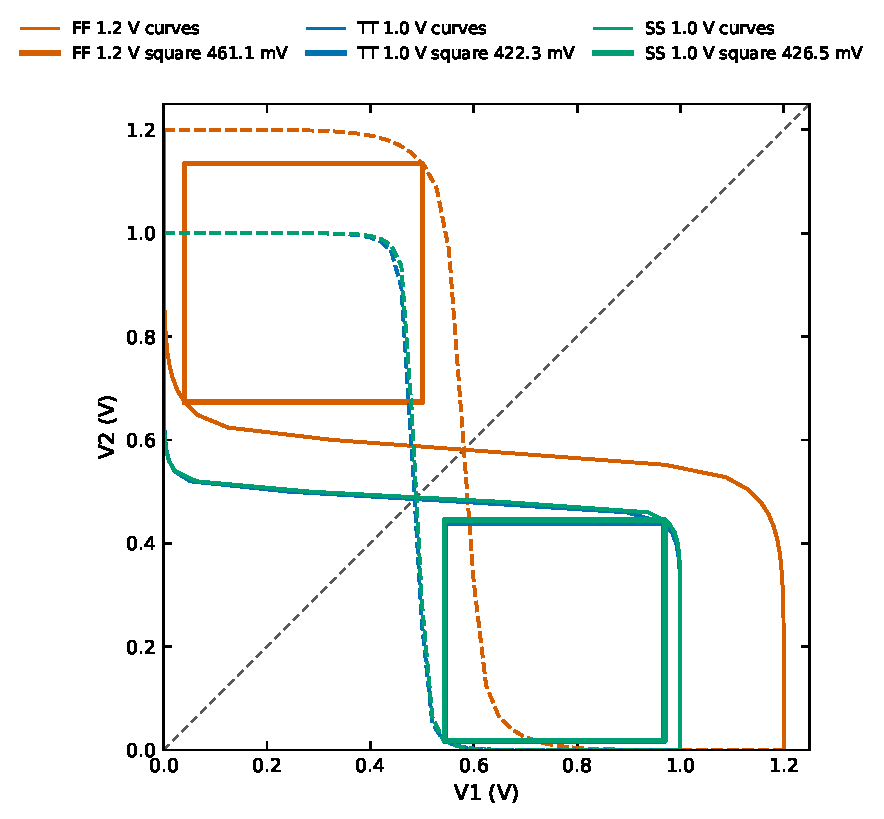
\includegraphics[width=0.9\columnwidth]{figures/baseline_hold_snm_all_corners.pdf}
\caption{Baseline hold-SNM butterfly overlays across corners.}\label{figA:baseline-hold}
\end{figure}

\begin{figure}[h]
\centering
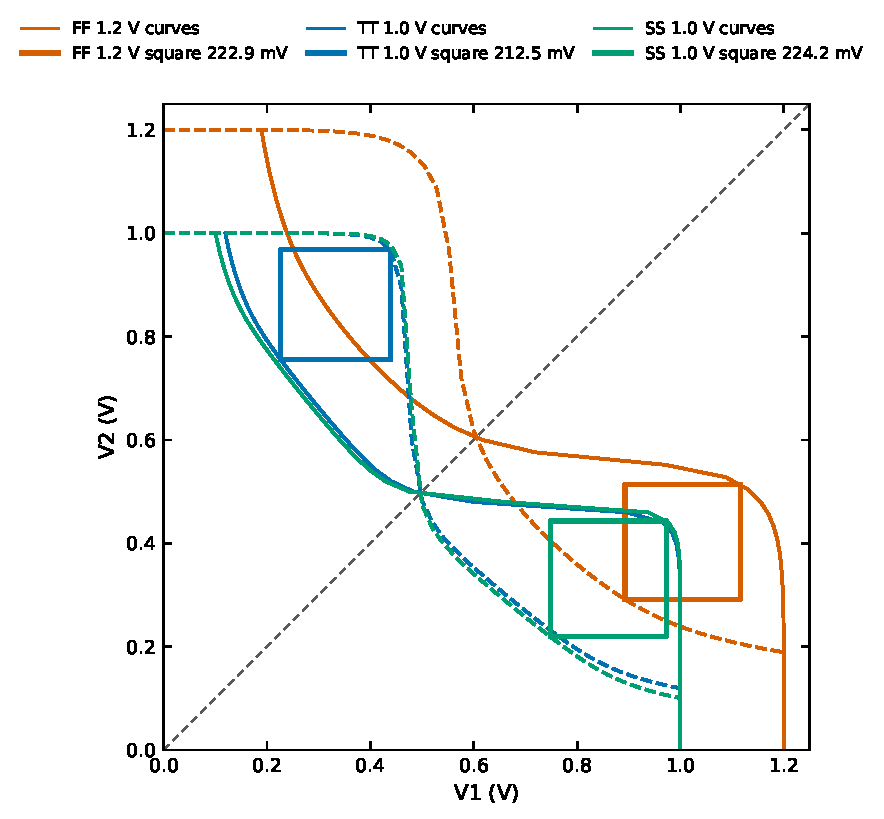
\includegraphics[width=0.9\columnwidth]{figures/baseline_read_snm_all_corners.pdf}
\caption{Baseline read-SNM butterfly overlays across corners.}\label{figA:baseline-read}
\end{figure}

\begin{figure}[h]
\centering
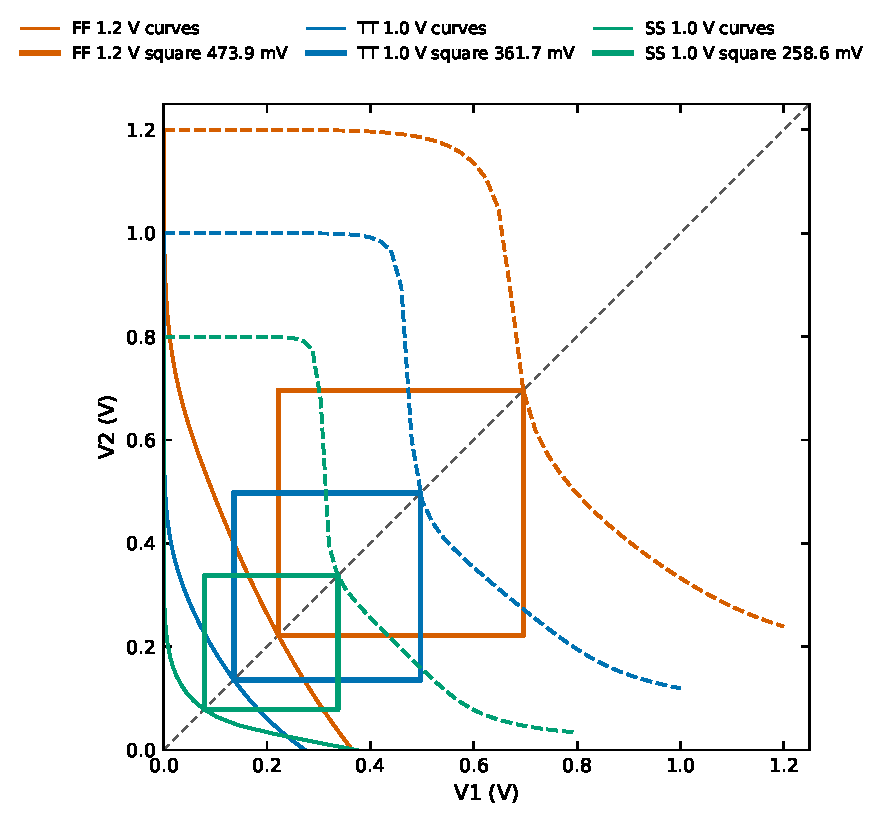
\includegraphics[width=0.9\columnwidth]{figures/baseline_write_nm_all_corners.pdf}
\caption{Baseline WNM butterfly overlays across corners.}\label{figA:baseline-wnm}
\end{figure}

\end{appendices}

\end{document}
